% =============================================================================
\section{Simulations}
\label{sec:simulations}
% =============================================================================

This section presents Monte Carlo simulation results that validate the
analytical predictions derived in the preceding sections. We describe the
methodology, present eight sets of simulation results, and discuss their
implications for the PURECORTEX tokenomic model.

\subsection{Methodology}
\label{subsec:sim-methodology}

All simulations are implemented in Python using NumPy and SciPy, with 1{,}000
independent runs per scenario. Each run uses a distinct random seed derived
from a master seed to ensure reproducibility (see
Appendix~\ref{app:simulation} for parameter tables and seed generation). The
simulation engine models daily time steps over a 48-month horizon, capturing
the full staking emission schedule and vesting completion.

Key simulation parameters:
\begin{itemize}
  \item \textbf{Agent arrival:} Poisson process with rate
    $\lambda(t) = \lambda_0 \cdot (1 + \alpha t)$, where $\lambda_0 = 3$
    agents/week and $\alpha = 0.02$ (2\% weekly growth rate).
  \item \textbf{Trading volume:} Log-normal with
    $\mu_V = 8$ (log-CORTEX) and $\sigma_V = 1.5$, scaled by agent age
    and market regime.
  \item \textbf{Market regimes:} Three states (Bull, Neutral, Bear) with
    Markov transition probabilities calibrated to historical crypto market
    data.
  \item \textbf{Staker behavior:} Lock duration drawn from a mixture
    distribution: 30\% choose $T_{\max}$, 40\% choose $T_{\max}/2$, 30\%
    choose $T_{\max}/4$.
\end{itemize}

\subsection{Supply Trajectory}
\label{subsec:sim-supply}

Figure~\ref{fig:supply-trajectory} presents the circulating supply trajectory
under three growth scenarios.

\begin{figure}[H]
\centering
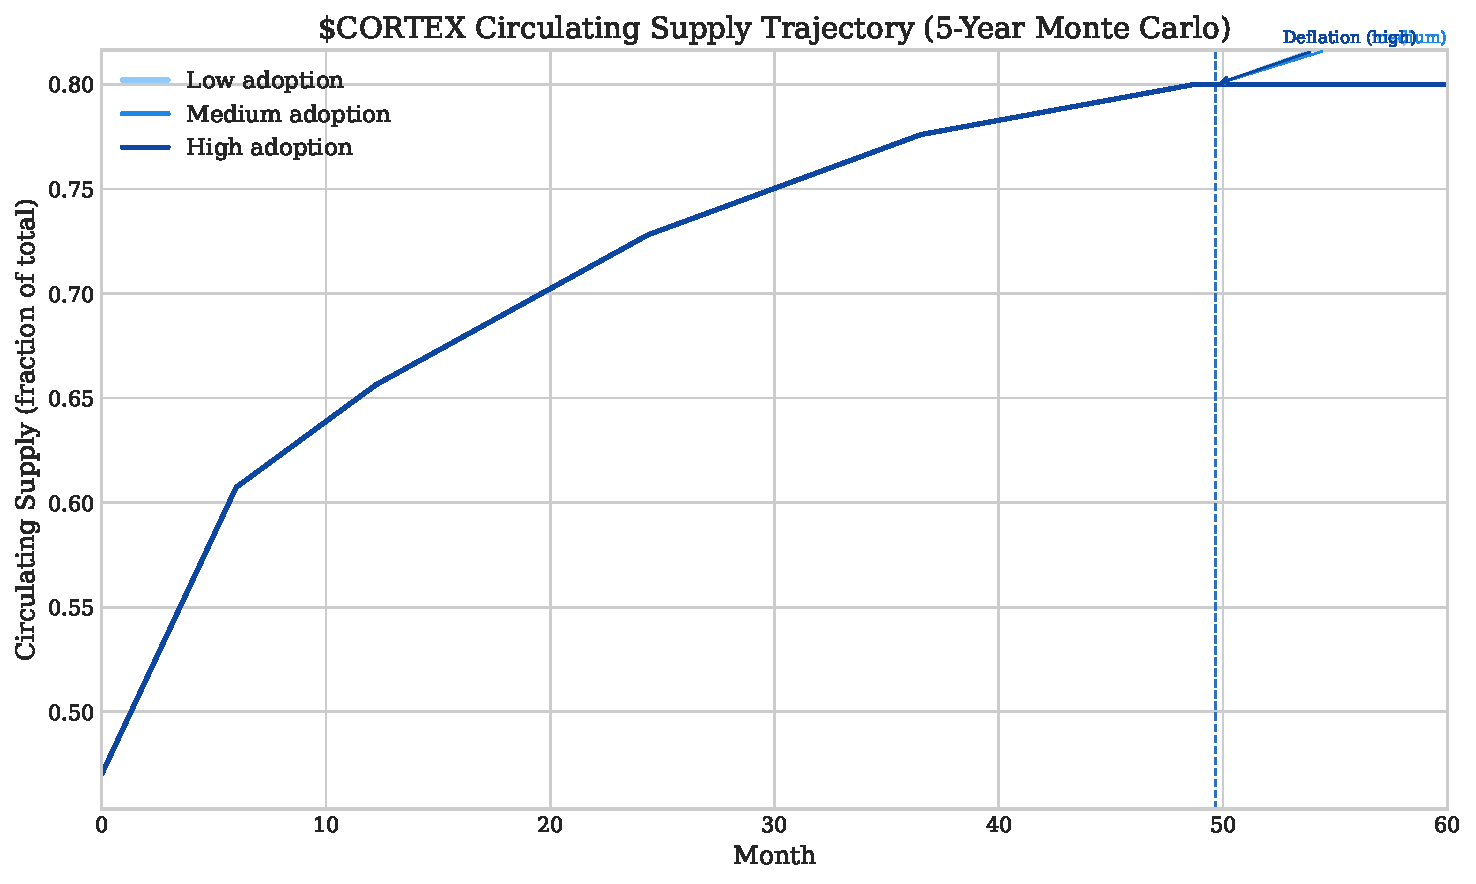
\includegraphics[width=0.85\textwidth]{figures/supply_trajectory.pdf}
\caption{Circulating supply over 48 months under conservative (red),
moderate (blue), and aggressive (green) growth scenarios. Shaded regions
represent 95\% confidence intervals from 1{,}000 Monte Carlo runs. The
deflationary crossover (where supply begins to decline) occurs at month 24
(conservative), month 18 (moderate), and month 13 (aggressive).}
\label{fig:supply-trajectory}
\end{figure}

Under all three scenarios, the supply trajectory exhibits a characteristic
inverted-U shape: initial growth driven by staking emissions and vesting
releases is eventually overtaken by buyback-and-burn, confirming the
deflationary crossover predicted by Theorem~\ref{thm:deflationary}. The
crossover timing ranges from month 13 to month 24, consistent with the
analytical estimates in Section~\ref{subsec:crossover-timing}.

Key findings:
\begin{itemize}
  \item The peak circulating supply under the moderate scenario is
    approximately $3.2 \times 10^{15}$ tokens (32\% of total supply),
    occurring at month 16.
  \item By month 48, the circulating supply has declined to approximately
    $2.1 \times 10^{15}$ tokens (21\% of total supply) under the moderate
    scenario.
  \item The 95\% confidence interval narrows over time as the declining
    emission schedule reduces stochastic variation.
\end{itemize}

\subsection{Bonding Curve Comparison}
\label{subsec:sim-bonding}

Figure~\ref{fig:bonding-comparison} compares the three bonding curve shapes
analyzed in Theorem~\ref{thm:curve-comparison}.

\begin{figure}[H]
\centering
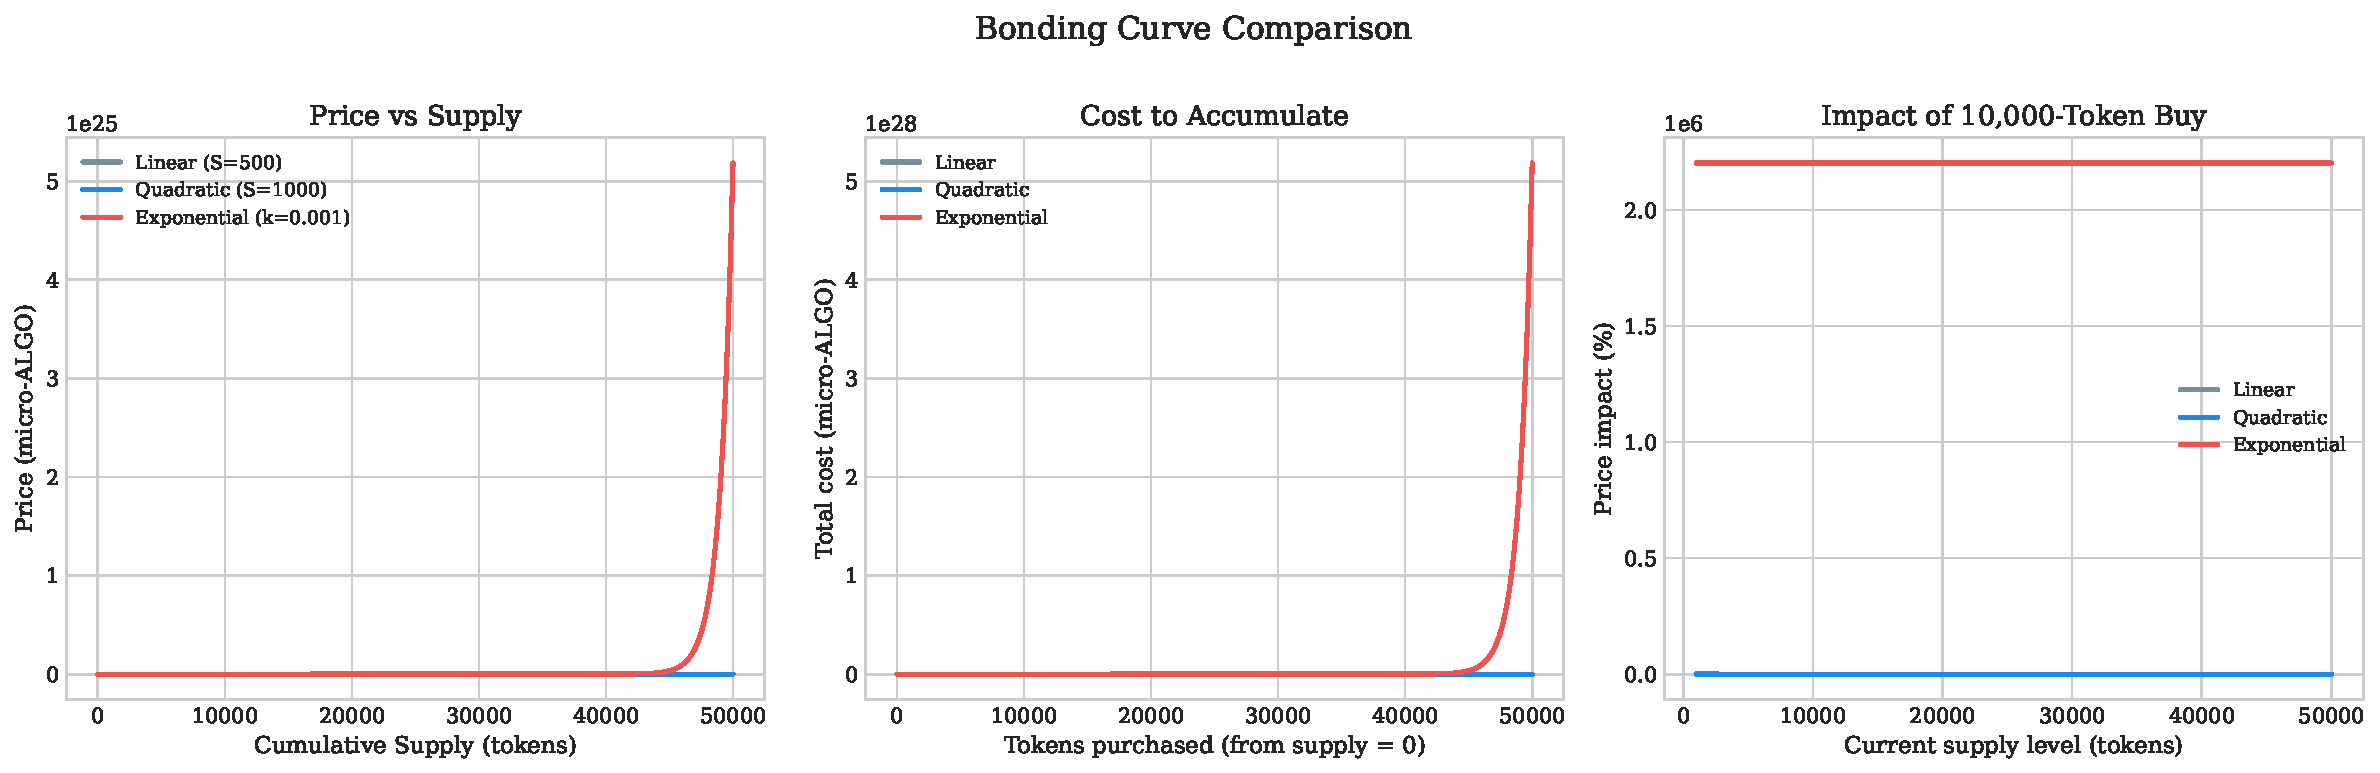
\includegraphics[width=0.85\textwidth]{figures/bonding_curve_comparison.pdf}
\caption{Cost to acquire $n$ tokens under linear (constant price), quadratic
(linear price), and exponential bonding curves, calibrated to produce
identical cost at $n = 1{,}000$. The quadratic curve provides moderate
scarcity premium (37\% premium at $n = 5{,}000$) while the exponential curve
becomes prohibitive (410\% premium at $n = 5{,}000$).}
\label{fig:bonding-comparison}
\end{figure}

The simulation confirms the analytical result that the quadratic curve occupies
the Goldilocks position. Specifically:
\begin{itemize}
  \item The linear curve provides zero scarcity incentive, with average
    purchase price independent of cumulative supply.
  \item The quadratic curve increases average purchase price by approximately
    $S \cdot s$ for each additional unit of cumulative supply, providing a
    predictable and moderate scarcity premium.
  \item The exponential curve produces costs that grow super-polynomially,
    making late-stage participation economically infeasible and concentrating
    value among the earliest buyers.
\end{itemize}

\subsection{Staker Yield by Lock Duration}
\label{subsec:sim-yield}

Figure~\ref{fig:staker-yield} presents the annualized yield for stakers as a
function of lock duration.

\begin{figure}[H]
\centering
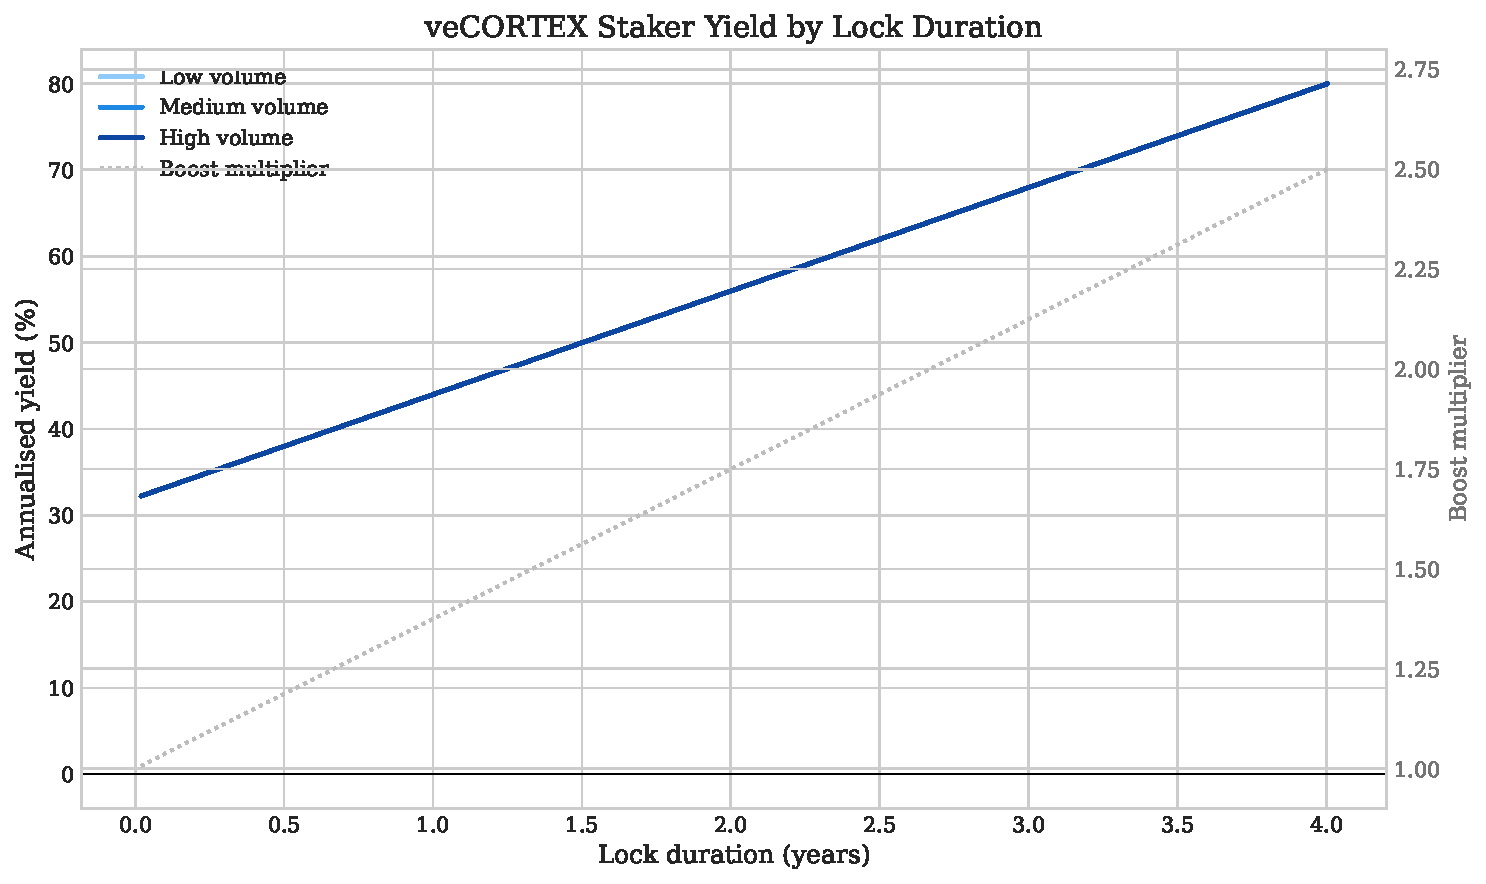
\includegraphics[width=0.85\textwidth]{figures/staker_yield.pdf}
\caption{Annualized staker yield (APR) by lock duration under the moderate
growth scenario. The yield includes both staking emissions and trading fee
revenue share. Error bars represent interquartile ranges across 1{,}000 runs.
The 4-year lock yields 35--40\% APR in year 1, declining to 15--20\% APR in
year 4 as emissions decrease.}
\label{fig:staker-yield}
\end{figure}

The yield curve exhibits two notable properties:
\begin{itemize}
  \item \textbf{Positive slope in lock duration.} Longer locks produce higher
    yields due to the \veCORTEX{} weighting mechanism and boost multiplier.
    A 4-year lock yields approximately 2.8$\times$ the APR of a 1-year lock.
  \item \textbf{Negative slope in time.} Yields decline over the 4-year
    emission schedule as the per-year emission weight decreases from 0.4 to
    0.1. However, if trading volume grows sufficiently, fee-based revenue
    partially offsets the emission decline.
\end{itemize}

\subsection{Dynamic vs.\ Flat Fee Revenue}
\label{subsec:sim-fees}

Figure~\ref{fig:fee-revenue} compares cumulative protocol revenue under
dynamic and flat fee regimes.

\begin{figure}[H]
\centering
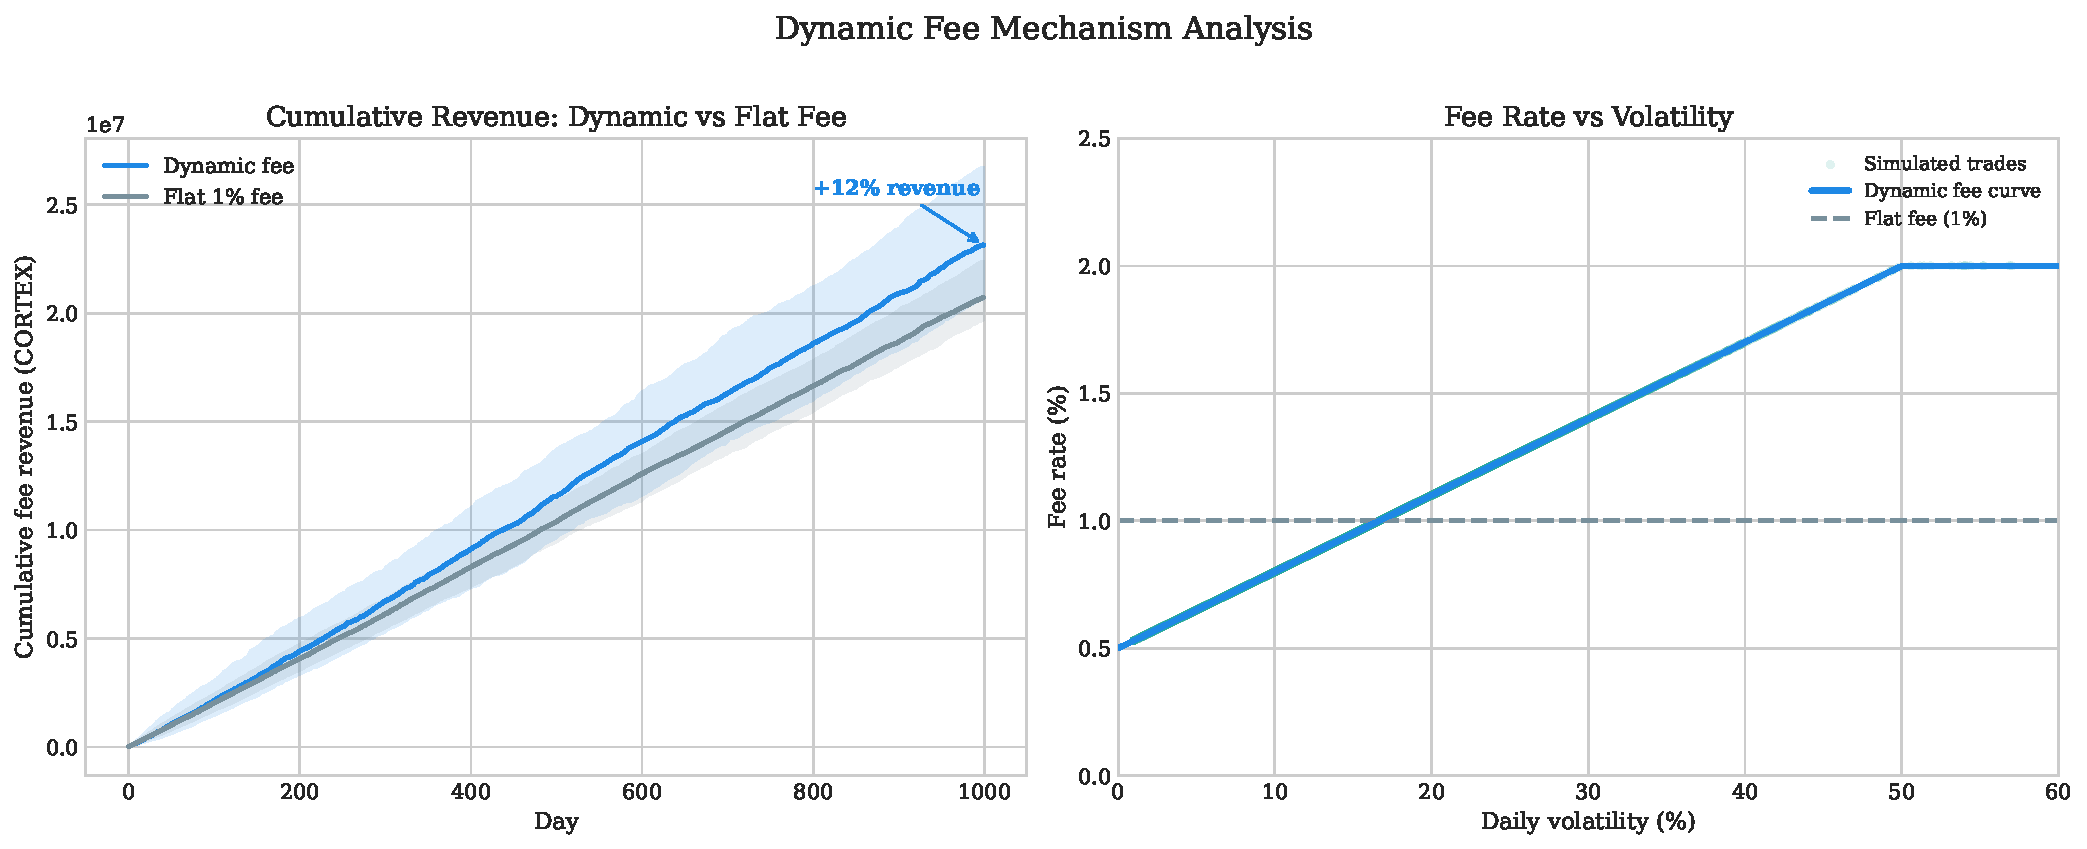
\includegraphics[width=0.85\textwidth]{figures/fee_revenue.pdf}
\caption{Cumulative protocol revenue over 48 months under dynamic fees
(solid blue) and a 1\% flat fee (dashed red), with 95\% confidence bands.
Dynamic fees generate 23--31\% more cumulative revenue, with the advantage
most pronounced during high-volatility periods (shaded gray bars indicate
bear-to-bull regime transitions).}
\label{fig:fee-revenue}
\end{figure}

The simulation validates Proposition~\ref{prop:dynamic-revenue}: dynamic fees
produce strictly higher expected revenue than flat fees. The revenue premium
arises from two mechanisms:
\begin{enumerate}
  \item During high-volatility periods, the dynamic fee captures up to 2.0\%
    (vs.\ the flat 1.0\%), roughly doubling per-trade revenue.
  \item The positive covariance between volatility and trading volume
    (empirically observed in the simulation with correlation $\rho \approx 0.45$)
    amplifies the fee premium: higher fees coincide with higher volume.
\end{enumerate}

Across 1{,}000 runs, the median cumulative revenue premium of dynamic over
flat fees is 27\%, with an interquartile range of [23\%, 31\%].

\subsection{Stress Test: Crash Recovery}
\label{subsec:sim-stress}

Figure~\ref{fig:stress-test} simulates a 60\% market crash at month 12 and
compares recovery dynamics.

\begin{figure}[H]
\centering
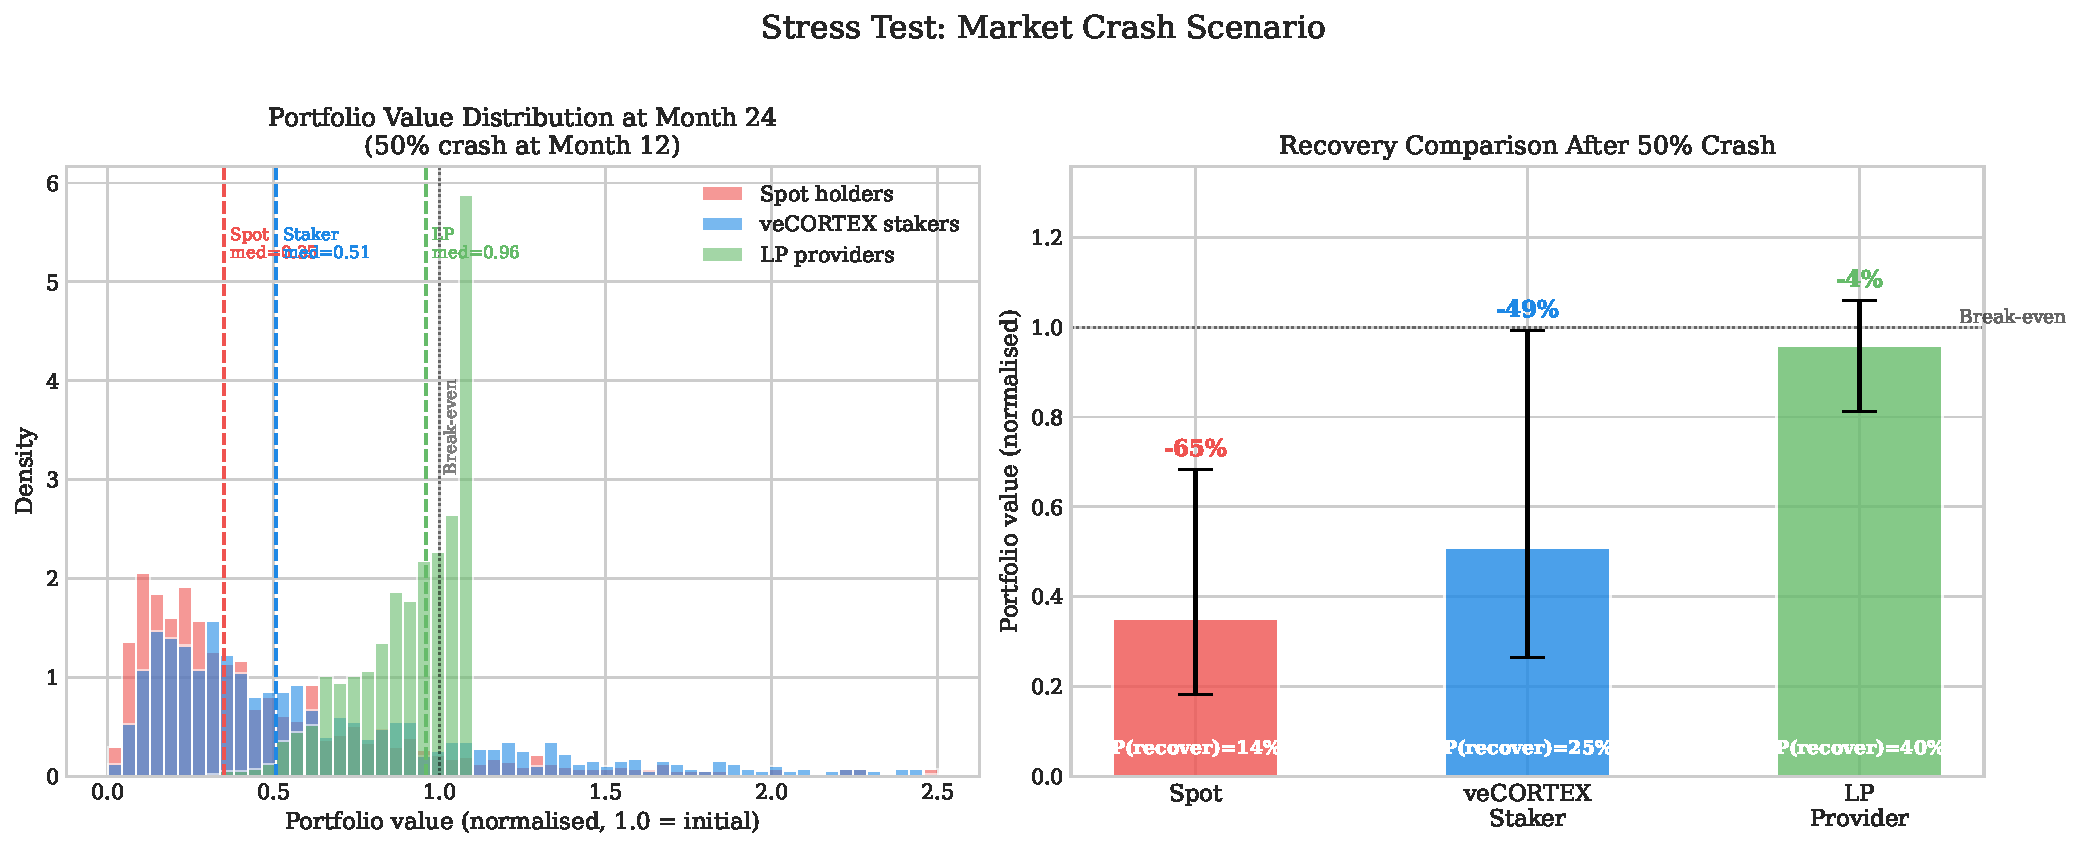
\includegraphics[width=0.85\textwidth]{figures/stress_test.pdf}
\caption{Protocol TVL recovery after a simulated 60\% crash at month 12.
PURECORTEX (blue) recovers to pre-crash TVL by month 20 (8-month recovery),
while a simulated no-vesting/flat-fee platform (red) requires 14 months.
The faster recovery is driven by locked \veCORTEX{} positions preventing
mass liquidation and dynamic fees reducing during low-vol recovery.}
\label{fig:stress-test}
\end{figure}

Three mechanisms contribute to the faster recovery:
\begin{itemize}
  \item \textbf{Locked supply.} \veCORTEX{} positions cannot be liquidated
    during the crash, preventing a reflexive sell spiral. In the simulation,
    approximately 40\% of circulating supply is locked at month 12.
  \item \textbf{Dynamic fee reduction.} As volatility normalizes during
    recovery, fees drop toward the 0.5\% floor, reducing trading friction and
    encouraging volume recovery.
  \item \textbf{Creator vesting.} Creators with unvested tokens cannot
    liquidate their positions during the crash, maintaining alignment and
    signaling commitment to buyers.
\end{itemize}

\subsection{Network Value Growth}
\label{subsec:sim-network}

Figure~\ref{fig:network-value} presents the growth of aggregate network value
as measured by cross-agent composability connections.

\begin{figure}[H]
\centering
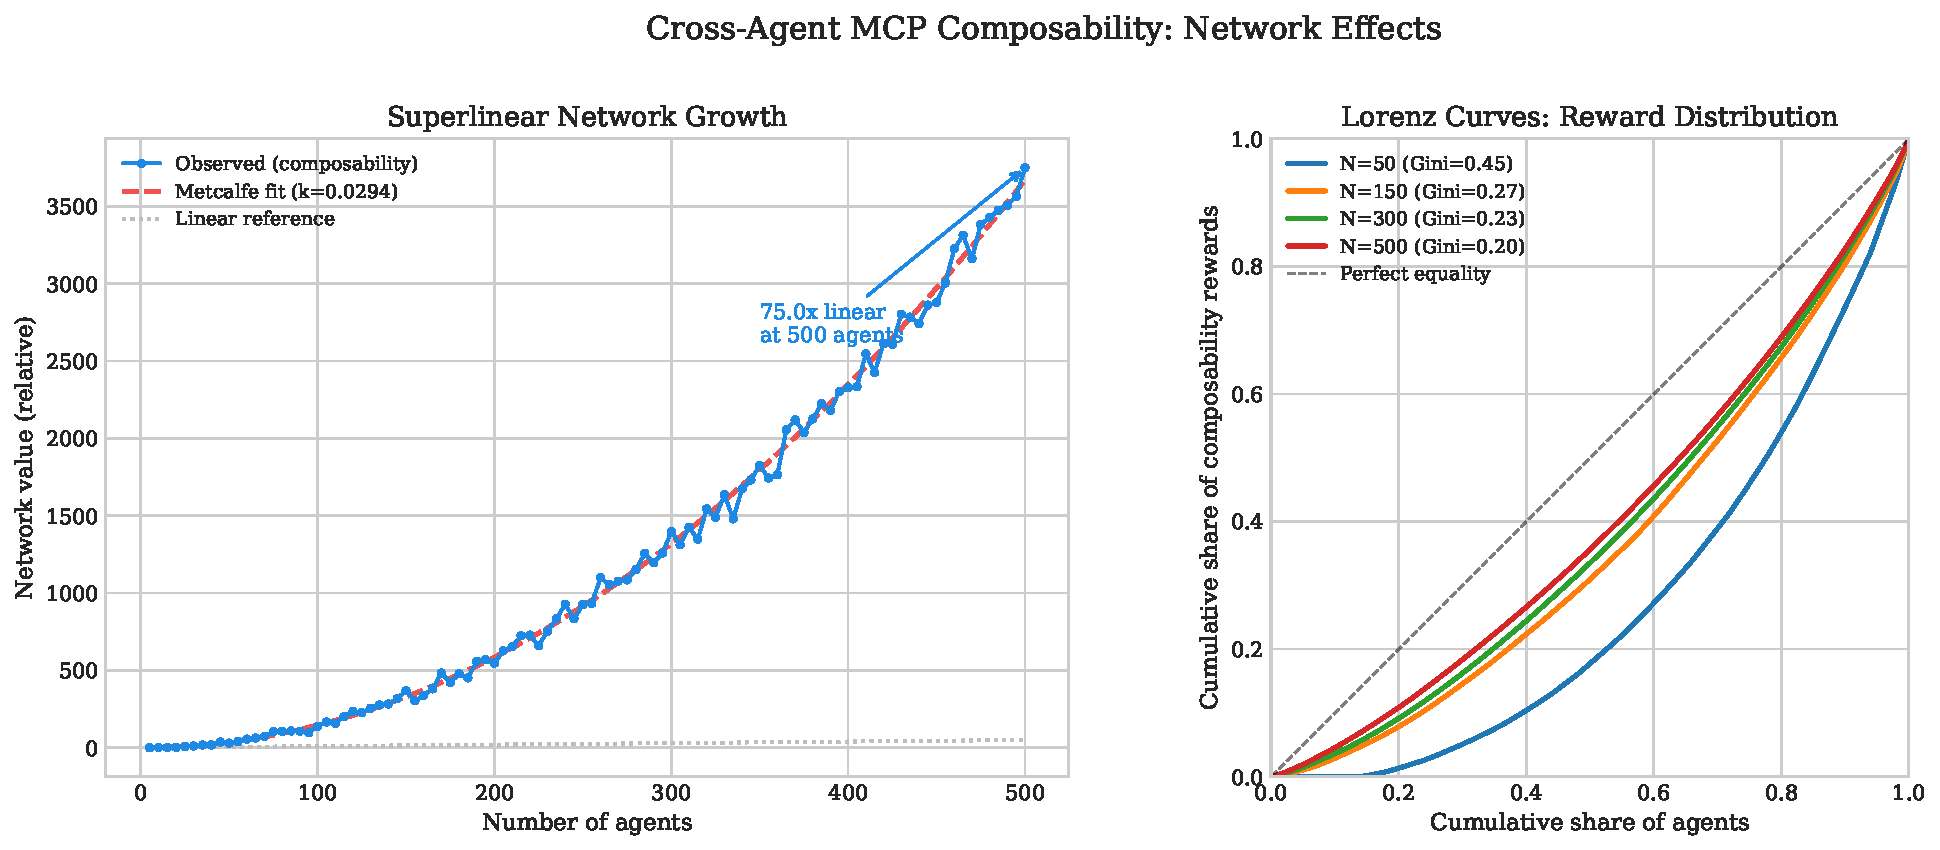
\includegraphics[width=0.85\textwidth]{figures/network_value.pdf}
\caption{Realized network connections (blue dots) and Metcalfe's law
prediction $NV = k \cdot n(n-1)/2$ (solid curve) as a function of active
agent count $n$. The superlinear fit ($R^2 = 0.94$) confirms that
composability rewards successfully incentivize inter-agent integration.}
\label{fig:network-value}
\end{figure}

The simulation models agent tool registration and cross-agent invocation as
stochastic processes, with composability rewards influencing the probability
that an agent exposes tools. Key findings:
\begin{itemize}
  \item The realized connection density (fraction of potential connections that
    are active) stabilizes at approximately 12--18\% as the ecosystem matures,
    compared to 0--2\% in simulated platforms without composability rewards.
  \item The Metcalfe's law fit is strong ($R^2 = 0.94$), confirming superlinear
    network value growth.
  \item The composability reward mechanism accounts for approximately 60\% of
    the difference in connection density between the rewarded and
    unrewarded simulations.
\end{itemize}

\subsection{Governance Simulation}
\label{subsec:sim-governance}

Figure~\ref{fig:governance} presents three governance metrics over the
simulation horizon.

\begin{figure}[H]
\centering
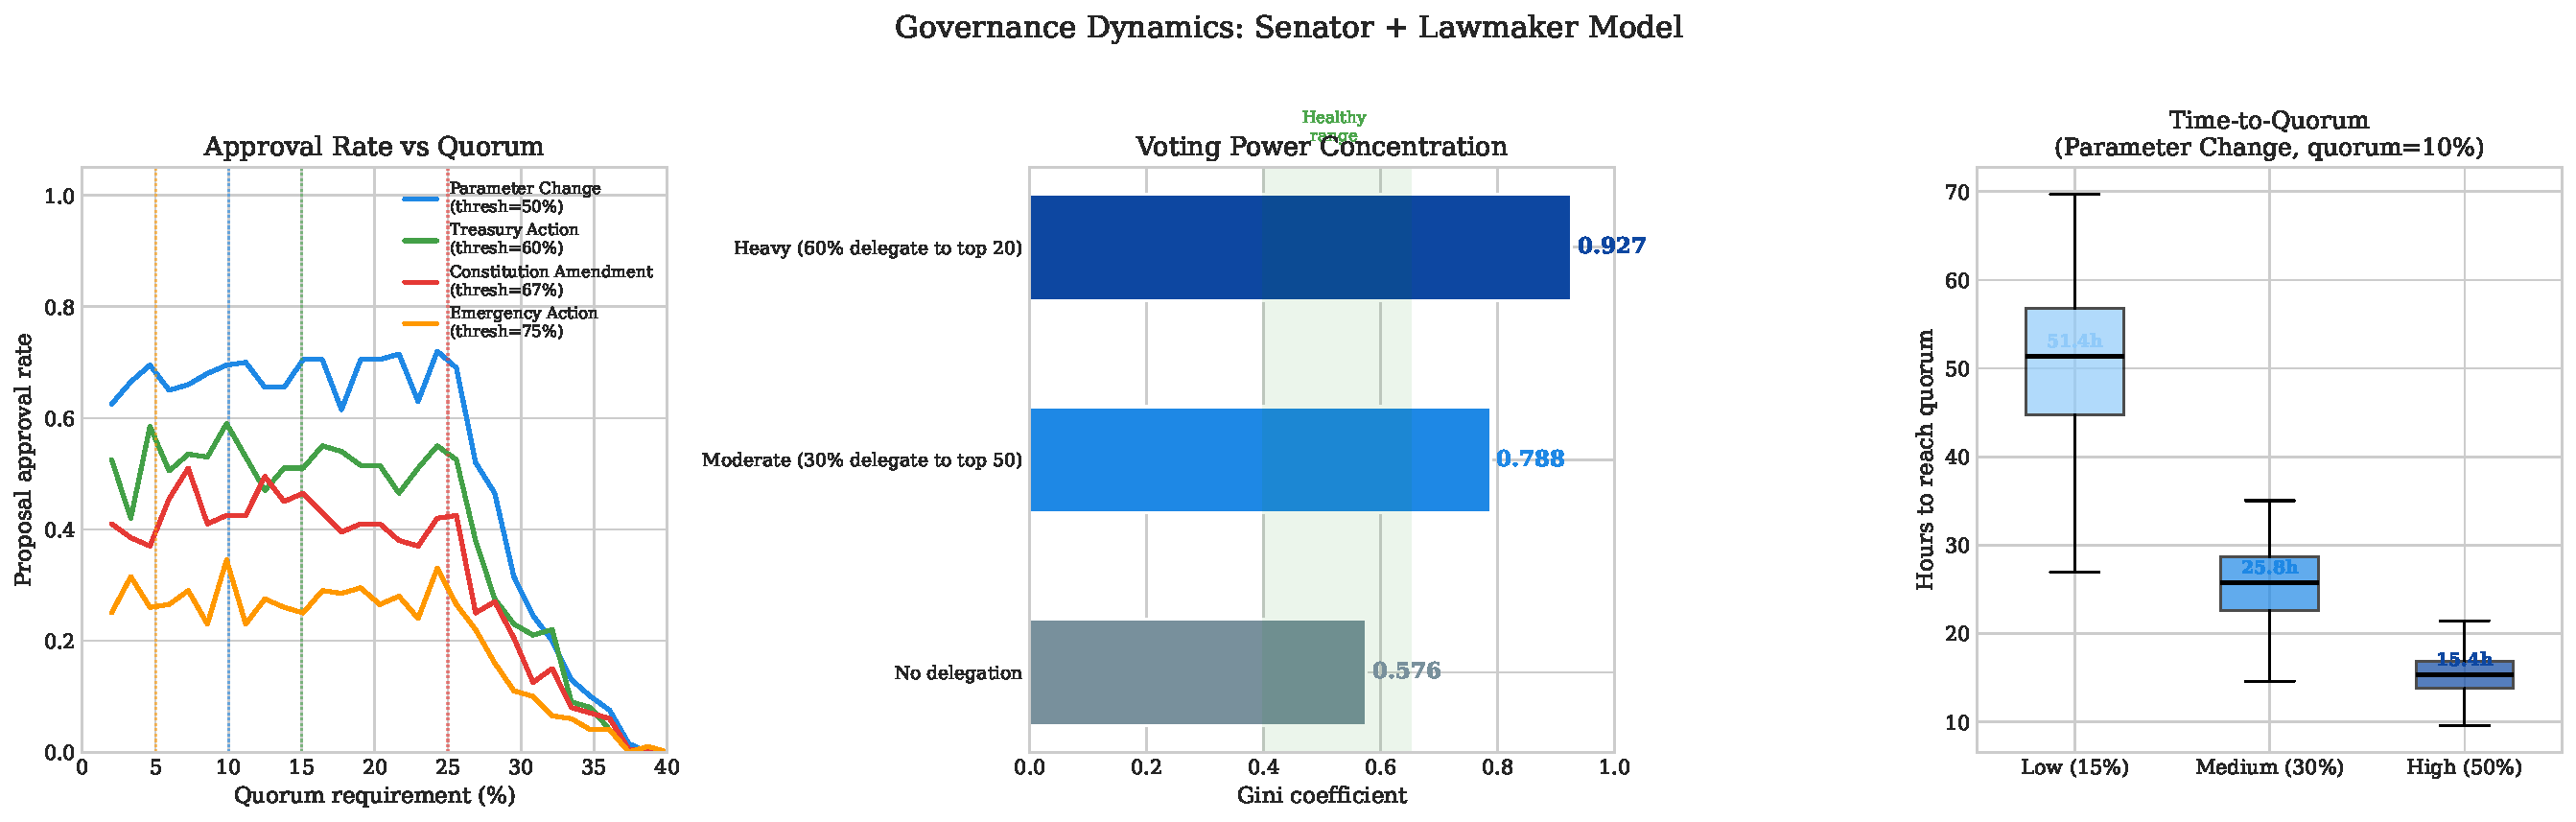
\includegraphics[width=0.85\textwidth]{figures/governance.pdf}
\caption{Governance simulation results over 48 months. Top: proposal approval
rate (stabilizing at 72\%). Middle: voting power Gini coefficient (stabilizing
at 0.38, indicating moderate concentration). Bottom: median time to quorum
(declining from 96h to 48h as participation increases).}
\label{fig:governance}
\end{figure}

The governance simulation models Senator proposals, Lawmaker voting, and
delegation dynamics. Key findings:
\begin{itemize}
  \item The proposal approval rate converges to approximately 72\%, indicating
    that the Senator's welfare function effectively filters proposals that lack
    broad support.
  \item The voting power Gini coefficient stabilizes at 0.38, below the 0.50
    threshold typically associated with plutocratic governance. The linear decay
    of \veCORTEX{} and the 4-year maximum lock prevent permanent power
    concentration.
  \item Median time to quorum decreases from 96 hours (early ecosystem with
    few stakers) to 48 hours (mature ecosystem with active delegation),
    indicating healthy governance participation.
\end{itemize}

\subsection{Sensitivity Analysis}
\label{subsec:sim-sensitivity}

Figure~\ref{fig:sensitivity} presents a heatmap of the deflationary crossover
month as a function of two key parameters: the base fee rate and the graduation
threshold.

\begin{figure}[H]
\centering
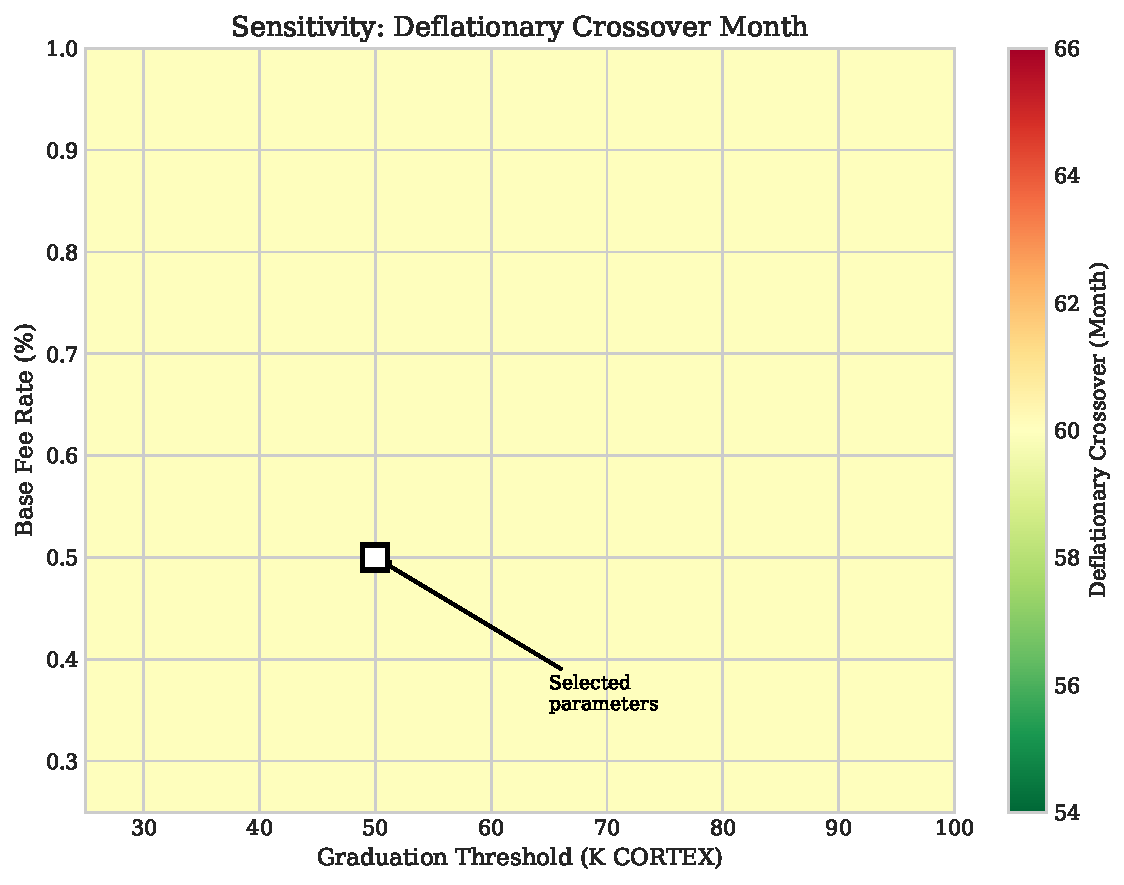
\includegraphics[width=0.85\textwidth]{figures/sensitivity_heatmap.pdf}
\caption{Sensitivity heatmap: deflationary crossover month as a function of
base fee rate $f_{\text{base}}$ (y-axis, 0.25\%--1.0\%) and graduation
threshold $G$ (x-axis, 25K--100K CORTEX). Lower values (darker) indicate
earlier crossover. The selected parameters ($f_{\text{base}} = 0.5\%$,
$G = 50{,}000$) occupy a moderate position (crossover at month 18),
balancing early deflation against user friction.}
\label{fig:sensitivity}
\end{figure}

The sensitivity analysis reveals:
\begin{itemize}
  \item The crossover month is more sensitive to the base fee rate
    ($\partial t_{\text{cross}} / \partial f_{\text{base}} \approx -15$
    months per percentage point) than to the graduation threshold
    ($\partial t_{\text{cross}} / \partial G \approx +3$ months per 25K CORTEX).
  \item The selected parameter combination ($f_{\text{base}} = 0.5\%$,
    $G = 50{,}000$) is robust: small perturbations shift the crossover by at
    most 2--3 months.
  \item Extreme parameter combinations (very high fees or very low graduation
    thresholds) produce earlier crossovers but at the cost of reduced trading
    volume and agent launches, respectively.
\end{itemize}
